\documentclass{article}
\usepackage[utf8]{inputenc}
\usepackage[margin=1in]{geometry}
\usepackage{array}
\usepackage{multirow}
\usepackage{makecell}
\usepackage{listings}
\usepackage{pdflscape}
\usepackage{graphicx}
\graphicspath{ {images/} }

\title{Schwap CPU Design Documentation}
\author{Charlie Fenoglio, Alexander Hirschfeld, Andrew McKee, and Wesley Van Pelt}
\date{Winter 2015/2016}

\begin{document}
\maketitle
\section{Registers}
	There are a total of 76 16-bit registers; 12 are fixed and 64 (spilt into 16 groups of 4) "schwapable" registers.  Some registers have alias names, see Section 6.3.1 for a list.
	\subsection{Register Names and Descriptions}
		\begin{center}
			\begin{tabular}{| c | c | c | c |}
				\hline
				    Name        & Number  & Description            & Saved Across Call? \\ \hline
				    \$z0        & 0       & The Value 0$^\dagger$  & -   \\ \hline
				    \$a0        & 1       & Assembler Temporary 0  & No  \\ \hline
				    \$a1        & 2       & Assembler Temporary 1  & No  \\ \hline
				    \$pc        & 3       & Program Counter$^\ddagger$& Yes \\ \hline
				    \$sp        & 4       & Stack Pointer          & Yes \\ \hline
				    \$ra        & 5       & Return Address         & Yes \\ \hline
				    \$s0 - \$s1 & 6 - 7   & User Saved Temporaries & Yes \\ \hline
				    \$t0 - \$t3 & 8 - 11  & User Temporaries       & No  \\ \hline
				    \$h0 - \$h3 & 12 - 15 & Schwap                 & -   \\
				\hline
			\end{tabular} \\
			$^\dagger$See Section 6.1.1-1 for details\\
			$^\ddagger$See Section 6.1.1-2 for details
		\end{center}
	\subsection{Schwap Registers}
		The "schwap" registers are registers that appear to be swapped using a command.  There is no data movement when schwapping, it only changes which registers the \$h0 - \$h3 refer to.  There are 8 groups the user can use for general purpose and 8 reserved groups.
		\subsubsection{Schwap Group Numbers, Descriptions, and Uses}
			\begin{center}
				\begin{tabular}{| c | c | c |}
					\hline
				    	Group Number & Uses                      & Saved Across Call? \\ \hline
					    0 - 3        & User Temporaries          & No \\ \hline
					    4 - 7        & User Saved Temporaries    & Yes\\ \hline
					    8            & Arguments 0 - 3           & No \\ \hline
					    9            & Return Values 0 - 3       & No \\ \hline
					    10 - 14      & Reserved For Future Use$^\dagger$ & -  \\ \hline
					    15           & Go to the last used group & -  \\
					\hline
				\end{tabular} \\
				$^\dagger$See Section 6.1.2-1 for details
			\end{center}
\newpage
\section{Instructions}
	All instructions are 16-bits.  The destination register is also used as a source unless otherwise noted.  All offsets are bit shifted left by 1 since all instructions are 2 bytes long.
	\subsection{Instruction Types and Bit Layouts}
		Instructions can be manually translated by putting the bits for each of the components of the instructions in the places listed by the diagrams for each type.  The OP codes, function codes, and types can by found on the "Core Instructions Summary" (2.2.1) table.  The destination and source are register numbers, which can be found under the "Register Names and Descriptions" (1.1) table.  Schwap group numbers can be found under the "Schwap Group Numbers, Descriptions, and Uses" (1.2.1) table.  The active schwap group is not preserved over a function call.  See Section 6.2.1 for notes on the types and layouts.
		\subsubsection{A-Type}
			\begin{center}
				\begin{tabular}{l r l r l r l r}
					\hline
					\multicolumn{2}{| p{2cm} |}{OP Code} & \multicolumn{2}{p{2cm}}{Destination} & \multicolumn{2}{| p{2cm} |}{Source} & \multicolumn{2}{p{2cm} |}{Func. Code} \\ \hline
					15 & 12 & 11 & 8 & 7 & 4 & 3 & 0
				\end{tabular}
				\begin{tabular}{l r l r l r l r}
					\hline
					\multicolumn{2}{| p{2cm} }{Immediate} & \multicolumn{2}{p{2cm}}{ } & \multicolumn{2}{ p{2cm} }{ } & \multicolumn{2}{p{2cm} |}{ } \\ \hline
					15 & & & & & & & 0
				\end{tabular}
			\end{center}
			Used for all ALU operations.  It consists of a 4-bit OP code, 4-bit destination, 4-bit source, and a 4-bit function code.  If the instruction has an immediate, it is inserted as the next instruction.
		\subsubsection{B-Type}
			\begin{center}
				\begin{tabular}{l r l r l r l r}
					\hline
					\multicolumn{2}{| p{2cm} |}{OP Code} & \multicolumn{2}{p{2cm}}{R0} & \multicolumn{2}{| p{2cm} |}{R1} & \multicolumn{2}{p{2cm} |}{Offset} \\ \hline
					15 & 12 & 11 & 8 & 7 & 4 & 3 & 0
				\end{tabular}
			\end{center}
			If it is being used for branching it consists of a 4-bit OP code, 4-bit 1st source (R0), 4-bit 2nd source (R1), and a 4-bit (unsigned) offset. If it is being used for reading from memory it consists of a 4-bit OP code, 4-bit destination (R0 not used as a source), 4-bit source (R1), and a 4-bit (unsigned) offset.  If it is being used for writing to memory it consists of a 4-bit OP code, 4-bit source (R0), 4-bit destination (R1), and a 4-bit (unsigned) offset.
		\subsubsection{H-Type}
			\begin{center}
				\begin{tabular}{l r l r l r l r}
					\hline
					\multicolumn{2}{| p{2cm} |}{OP Code} & \multicolumn{2}{p{2cm}}{ } & \multicolumn{2}{p{2cm}}{ } & \multicolumn{2}{| p{2cm} |}{Group} \\ \hline
					15 & 12 & & & & & 3 & 0
				\end{tabular}
			\end{center}
			Used for schwapping and sudo.  It consists of a 4-bit OP code, 8 unused bits, and a 4-bit schwap group number or sudo use case.
		\subsubsection{J-Type}
			Used for jumping.  It consists of a 4-bit OP code, 4-bit source, and an 8-bit (signed) offset.
			\begin{center}
				\begin{tabular}{l r l r l r l r}
					\hline
					\multicolumn{2}{| p{2cm} |}{OP Code} & \multicolumn{2}{p{2cm}}{Source} & \multicolumn{2}{| p{2cm} }{Offset} & \multicolumn{2}{p{2cm} |}{ } \\ \hline
					15 & 12 & 11 & 8 & 7 & & & 0
				\end{tabular}
			\end{center}
	\subsection{Core Instructions}
		Some instructions have alias names, see Section 6.3.2 for a list. [dest], [src], [src0], [src1] all refer to a register in the register file, for example \$t0.  "NAM" stands for the name of the instruction (for example, "and").  "OP" stands for whatever the op would be (for example, "\&").
		\subsubsection{A-Type}
			\begin{center} \begin{tabular}{| c | c | c |} \hline
				\thead{Function \\ Code} & Name & Description \\ \hline
				0x0 & and & \thead{Bitwise ands 2 values}\\ \hline
			    0x1 & orr & \thead{Bitwise ors 2 values}\\ \hline
			    0x2 & xor & \thead{Bitwise xors 2 values}\\ \hline
			    0x3 & not & \thead{Bitwise nots the value}\\ \hline
			    0x4 & tsc & \thead{Converts a number to 2's compliment}\\ \hline
			    0x5 & slt & \thead{Set less than}\\ \hline
			    0x6 & sll & \thead{Left logical bit shift}\\ \hline
			    0x7 & srl & \thead{Right logical bit shift}\\ \hline
			    0x8 & sra & \thead{Right arithmetic bit shift}\\ \hline
			    0x9 & add & \thead{Adds 2 values}\\ \hline
			    0xA & sub & \thead{Subtracts 2 values}\\ \hline
			    0xF & cpy & \thead{Copies the value in one register to another}\\ \hline
			\end{tabular} \end{center}
			All A-Type instructions, except for not, tsc, slt, and cpy, follow the syntax in the first section of the table below.  Those three can be found in the next sections.
			\begin{center} \begin{tabular}{| c | l | c | c |} \hline
				\thead{OP\\Code}     & Syntax                       & Meaning & Description \\ \hline
				0x0                  & NAM [dest] [src]             & \thead{dest $=$ dest OP src} & \thead{OPs the values in registers [dest] and [src]}\\ \hline
				\multirow{3}{*}{0x1} & NAM [dest] [src] [immediate] & \thead{src $=$ immediate \\ dest $=$ dest OP src} & \thead{Loads the immediate into the register [src] and \\ then OPs the values in registers [dest] and [src]}\\ \cline{2-4}
				                     & NAM [dest] [immediate]       & \thead{dest $=$ dest OP immediate} & \thead{OPs the immediate and the value in the \\ register [dest]}\\ \hline \hline
				0x0                  & not [dest]                   & \thead{dest $=$ $\sim$dest} & \thead{Bitwise nots the value in the register [dest]}\\ \hline
				0x1                  & not [immediate]              & \thead{dest $=$ $\sim$immediate} & \thead{Bitwise nots the immediate and puts the\\result in the register [dest]}\\ \hline \hline
				0x0                  & tsc [dest]                   & \thead{dest $=$ $\sim$dest + 1} & \thead{Converts the value in the register [dest]\\to 2's compliment}\\ \hline
				\multirow{3}{*}{0x1} & tsc [dest] [src] [immediate] & \thead{src $=$ immediate \\ dest $=$ $\sim$src + 1} & \thead{Loads the immediate into the register [src] \\ and then converts the value in register [src] \\ to 2's compliment and stores into [dest]}\\ \cline{2-4}
						             & tsc [dest] [immediate]       & \thead{dest $=$ $\sim$immediate + 1} & \thead{Converts the immediate to 2's compliment \\ and stores into the register [dest]}\\ \hline \hline
				0x0                  & slt [dest] [src]             & \thead{dest $=$ (dest $<$ src) ? 1 : 0} & \thead{If [dest] $<$ [src], then [dest] gets set to 1 \\ If [dest] $\geq$ [src], then [dest] gets set to 0}\\ \hline
				\multirow{3}{*}{0x1} & slt [dest] [src] [immediate] & \thead{src $=$ immediate \\ dest $=$ (dest $<$ src) ? 1 : 0} & \thead{Loads the immediate into the register [src] then \\ If [dest] $<$ [src], then [dest] gets set to 1 \\ If [dest] $\geq$ [src], then [dest] gets set to 0}\\ \cline{2-4}
						             & slt [dest] [immediate]       & \thead{dest $=$ \\ (dest $<$ immediate) ? 1 : 0} & \thead{If [dest] $<$ [immediate], then [dest] gets set to 1 \\ If [dest] $\geq$ [immediate], then [dest] gets set to 0}\\ \hline \hline
				0x0                  & cpy [dest] [src]             & \thead{dest $=$ src} & \thead{Copies the value the in register [src] into [dest]}\\ \hline
				0x1                  & cpy [dest] [immediate]       & \thead{dest $=$ immediate} & \thead{Loads the immediate into the register [dest]}\\ \hline
			\end{tabular} \end{center}
		\subsubsection{B-Type}
			\begin{center} \begin{tabular}{| c | c | c |} \hline
				\thead{OP \\ Code} & Name & Description \\ \hline
				 0x2 & beq  & \thead{Branches if the 2 values are equal}\\ \hline
				 0x3 & bne  & \thead{Branches if the 2 values are not equal}\\ \hline
				 0x4 & bgt  & \thead{Branches if value0 $>$ value1}\\ \hline
				 0x5 & blt  & \thead{Branches if value0 $<$ value1}\\ \hline
				 0x7 & r    & \thead{Reads the value in memory into a register}\\ \hline
				 0x8 & w    & \thead{Writes the value in a register into memory}\\ \hline
			\end{tabular} \end{center}
			The four different types of branches all follow the same syntax, "bnh" represents any branch name and "***" represents the condition.  They will become pseudo instructions iff branching up, or down more than 16 instructions.  Read and write each have their own syntaxes.  [offset] is not a register, it is an immediate.
			\begin{center} \begin{tabular}{| l | c | c |} \hline
				Syntax & Meaning & Description \\ \hline
				bnh [src0] [src1] label  & \thead{if(src0 *** src1) goto label} & \thead{If [src0] *** [src1], branch to label}\\ \hline
				r [dest] [offset]([src]) & \thead{dest $=$ Mem[src + offset$<<$1]} & \thead{Reads the data in the address of [src] + [offset] \\ in memory into [dest]}\\ \hline
				w [offset]([dest]) [src] & \thead{Mem[dest + offset<<1] $=$ src} & \thead{Writes the data in the address of [dest] + [offset] \\ in memory from [src]}\\ \hline
			\end{tabular} \end{center}
		\subsubsection{H-Type}
			\begin{center} \begin{tabular}{| c | c | l | c |} \hline
				\thead{OP \\ Code} & Name & Syntax & Description \\ \hline
				 0xE & rsh  & rsh [group] & \thead{Changes the schwap group number to [group], \\ these numbers can be found in the table in 1.2.1}\\ \hline
				 0xF & sudo & sudo [code] & \thead{Sames as syscall in MIPS} \\ \hline
			\end{tabular} \end{center}
		\subsubsection{J-Type}
			\begin{center} \begin{tabular}{| c | c | l | c | c |} \hline
				\thead{OP \\ Code} & Name & Syntax & Meaning & Description \\ \hline
				 0x6 & jr & jr [offset]([dest]) & \thead{pc $=$ dest + offset$<<$1} & \thead{Jumps to the instruction at the address in [dest] + [offset]}\\ \hline
			\end{tabular} \end{center}
	\subsection{Pseudo Instructions}
		There are two types of pseudo instructions.  One are instructions which are always pseudo instructions, the other are sometimes pseudo depending on the conditions.  Some instructions have alias names, see Section 6.3.2 for a list.
		\subsubsection{Always Pseudo Instructions}
			\begin{center} \begin{tabular}{| c | c | c | c |} \hline
				Name & Syntax    & Actual Code & Description \\ \hline
				j    & j label   & \thead{cpy \$a0 [label pc] \\ jr 0(\$a0)} & \thead{Jumps to the instruction at label}\\ \hline
				jal  & jal label & \thead{cpy \$ra \$pc \\ j [label]} & \thead{Stores the return address and then jumps to the label} \\ \hline
				bge  & bge [src0] [src1] label & \thead{cpy \$a0 [src0] \\ slt \$a0 [src1] \\ beq \$a0 \$z0 label} & \thead{If [src0] $\geq$ [src1], branch to label} \\ \hline
				ble  & ble [src0] [src1] label & \thead{cpy \$a0 [src1] \\ slt \$a0 [src0] \\ beq \$a0 \$z0 label} & \thead{If [src0] $\leq$ [src1], branch to label} \\ \hline
			\end{tabular} \end{center}
		\subsubsection{Conditional Pseudo Instructions}
			\begin{center} \begin{tabular}{| c | c | c | c |} \hline
				Name & Syntax                    & Actual Code & Condition \\ \hline
				beq  & beq [src0] [src1] label & \thead{bnq [src0] [src1] Next \\ j label \\ Next:} & \thead{Branching up or branching down \\ more than 16 instructions}\\ \hline
				bne  & bne [src0] [src1] label & \thead{beq [src0] [src1] Next \\ j label \\ Next:} & \thead{Branching up or branching down \\ more than 16 instructions}\\ \hline
				bgt  & bgt [src0] [src1] label & \thead{blt [src0] [src1] Next \\ j label \\ Next:} & \thead{Branching up or branching down \\ more than 16 instructions}\\ \hline
				blt  & blt [src0] [src1] label & \thead{bgt [src0] [src1] Next \\ j label \\ Next:} & \thead{Branching up or branching down \\ more than 16 instructions}\\ \hline
			\end{tabular} \end{center}
\section{RTL and Datapath}
	\subsection{Components}
		\subsubsection{Single 16-bit Register}
			\begin{center} \begin{tabular}{| l | l | c |} \hline 
				I/O & Name & Size \\ \hline 
				In  & in  & 16 \\ \hline
				Out & out & 16 \\ \hline
				Control & write & 1 \\ \hline
			\end{tabular} \end{center}
			\begin{center} \begin{tabular}{| l | c |} \hline 
				\multicolumn{2}{|c|}{Used as:} \\ \hline 
				IR       & \thead{Stores the 16-bit instruction that comes from memory} \\ \hline
				NextInst & \thead{Stores the next 16-bit instruction that comes from memory} \\ \hline
				PC       & \thead{Program Counter} \\ \hline
				R0       & \thead{Stores the value that comes out of reg0} \\ \hline
				R1       & \thead{Stores the value that comes out of reg1} \\ \hline
				ALUout   & \thead{Stores the value that comes out of the ALU} \\ \hline
				PCtemp   & \thead{Stores the value that comes out of ALUout for PC if needed} \\ \hline
				MemRead  & \thead{Same as IR, but is used for values} \\ \hline
			\end{tabular} \end{center}
		\subsubsection{Single 4-bit Register}
			\begin{center} \begin{tabular}{| l | l | c |} \hline 
				I/O & Name & Size \\ \hline 
				In  & in   & 4 \\ \hline
				Out & out  & 4 \\ \hline
				Control & writable & 1 \\ \hline
			\end{tabular} \end{center}
			\begin{center} \begin{tabular}{| l | c |} \hline 
				\multicolumn{2}{|c|}{Used as:} \\ \hline 
				Hreg & \thead{Stores IR[3:0]} \\ \hline
				SchLatch & \thead{Stores schwap group number} \\ \hline
			\end{tabular} \end{center}
		\subsubsection{SE$<<$1}
			\begin{center} Sign extends and then shifts it to the left 1 \end{center}
			\begin{center} \begin{tabular}{| l | l | c |} \hline 
				I/O & Name & Size \\ \hline 
				In  & in   & * \\ \hline
				Out & out  & * \\ \hline
			\end{tabular} \end{center}
		\subsubsection{16-bit Adder}
			\begin{center} \begin{tabular}{| l | l | c | l |} \hline 
				I/O & Name     & Size & Description \\ \hline 
				In  & A        & 16   & First input \\ \hline
				In  & B        & 16   & Second input \\ \hline
				Out & R        & 16   & Result \\ \hline
			\end{tabular} \end{center}
		\subsubsection{ALU}
			\begin{center} \begin{tabular}{| l | l | c | l |} \hline 
				I/O & Name     & Size & Description \\ \hline 
				In  & A        & 16   & First input \\ \hline
				In  & B        & 16   & Second input \\ \hline
				Out & R        & 16   & Result \\ \hline
				Out & zero     & 1    & If result is 0 \\ \hline
				Out & overflow & 1    & If there is overflow \\ \hline
				Control & op   & 4    & Operation code \\ \hline
			\end{tabular} \end{center}
		\subsubsection{Register File}
			\begin{center} \begin{tabular}{| l | l | c | l |} \hline
				I/O & Name       & Size & Description \\ \hline 
				In  & regID0     & 4    & ID for first register \\ \hline
				In  & regID1     & 4    & ID for second register \\ \hline
				In  & ImmIn0     & 16   & Data to write to regID1 \\ \hline
				Out & regOut0    & 16   & Data from regID0 \\ \hline
				Out & regOut1    & 16   & Data from regID1 \\ \hline
				Control & RegWrite & 1  & If data can be written to regID1\\ \hline
			\end{tabular} \end{center}
		\subsubsection{Main Memory}
			\begin{center} \begin{tabular}{| l | l | c | l |} \hline 
				I/O & Name  & Size & Description \\ \hline 
				In  & Addr0 & 16   & Address for data\\ \hline
				In  & Addr1 & 16   & Address for data\\ \hline
				In  & Store & 16   & Stores data at Addr0\\ \hline
				Out & Out0  & 16   & Data at Addr0 \\ \hline
				Out & Out1  & 16   & Data at Addr1 \\ \hline
				Control & memRead  & 1 & Set to 1 when data is to be read\\ \hline
				Control & memWrite & 1 & Set to 1 when data is to be written\\ \hline
			\end{tabular} \end{center}
		\subsubsection{Other Control Signals Not Listed}
			\begin{itemize}
				\item[PCSrc:] Where PC will get it's new value from
				\item[PCWrite:] Set to 1 if the PC should write the data on its input
				\item[Addr0src:] Where Addr0 will be getting its input from
				\item[RegStore:] Where ImmIn0 will be getting its input from
				\item[Imm:] If R1 should have an immediate loaded into it
				\item[ALUSrc0:] Where the first input of the ALU will be coming from
				\item[ALUSrc1:] Where the second input of the ALU will be coming from
				\item[ALUOpContr:] If the function code or ALUContr will decide the ALU op
				\item[ALUContr:] ALU op from the control unit
			\end{itemize}
	\newpage \begin{landscape}
	\subsection{Summary Charts}
		\subsubsection{RTL}
			\begin{center} \begin{tabular}{| c | c | c | c | c | c | c | c |} \hline
				\multirow{2}{*}{Step} & \multirow{2}{*}{A-Type} & \multicolumn{3}{c|}{B-Type} & \multicolumn{2}{c|}{H-Type} & \multirow{2}{*}{J-Type} \\ \cline{3-7}
				& & Branches & Read & Write & Schwap & Sudo & \\ \hline
				\thead{Get \\ instruction} & \multicolumn{7}{c|}{\thead{IR = MEM[PC] \\ NextInst = MEM[PC+2] \\ PC += 2}} \\ \hline
				\thead{Decode ins-\\truction and \\ get stuff from \\ registers} & \multicolumn{7}{c|}{\thead{R0 = reg\#IR[8:11] \\ if(IR[3:0]==0x1) \{R1 = NextInst; PC += 2\} else \{R1 = reg\#IR[7:4]\} \\ ALUout = PC + SE(IR[15:12]) \\ Hreg = IR[3:0]}} \\ \hline
				\thead{Do \\ computation} & \thead{ALUout = R0 aluop R1} & \thead{if(R0 aluop R1 == 0) \\ PC = ALUout} & \multicolumn{2}{c|}{\thead{ALUout = R1 + SE(Hreg$<<$1)}} & \thead{SchLatch\\= Hreg} & \thead{Change on\\Code\#} & \thead{PC = R0+\\SE(IR[7:0]$<<$1)} \\ \hline
				\thead{Output} & \thead{R0 in reg. file = ALUout} & & \thead{MemRead = MEM[ALUout]} & \thead{MEM[ALUout] = R0} & \multicolumn{3}{c|}{ } \\ \hline
				\thead{Output 2} & \multicolumn{2}{c|}{ } & \thead{R0 in reg. file = MemRead} & \multicolumn{4}{c|}{ } \\ \hline
			\end{tabular} \end{center}
		\subsubsection{Datapath}
			\begin{center}
				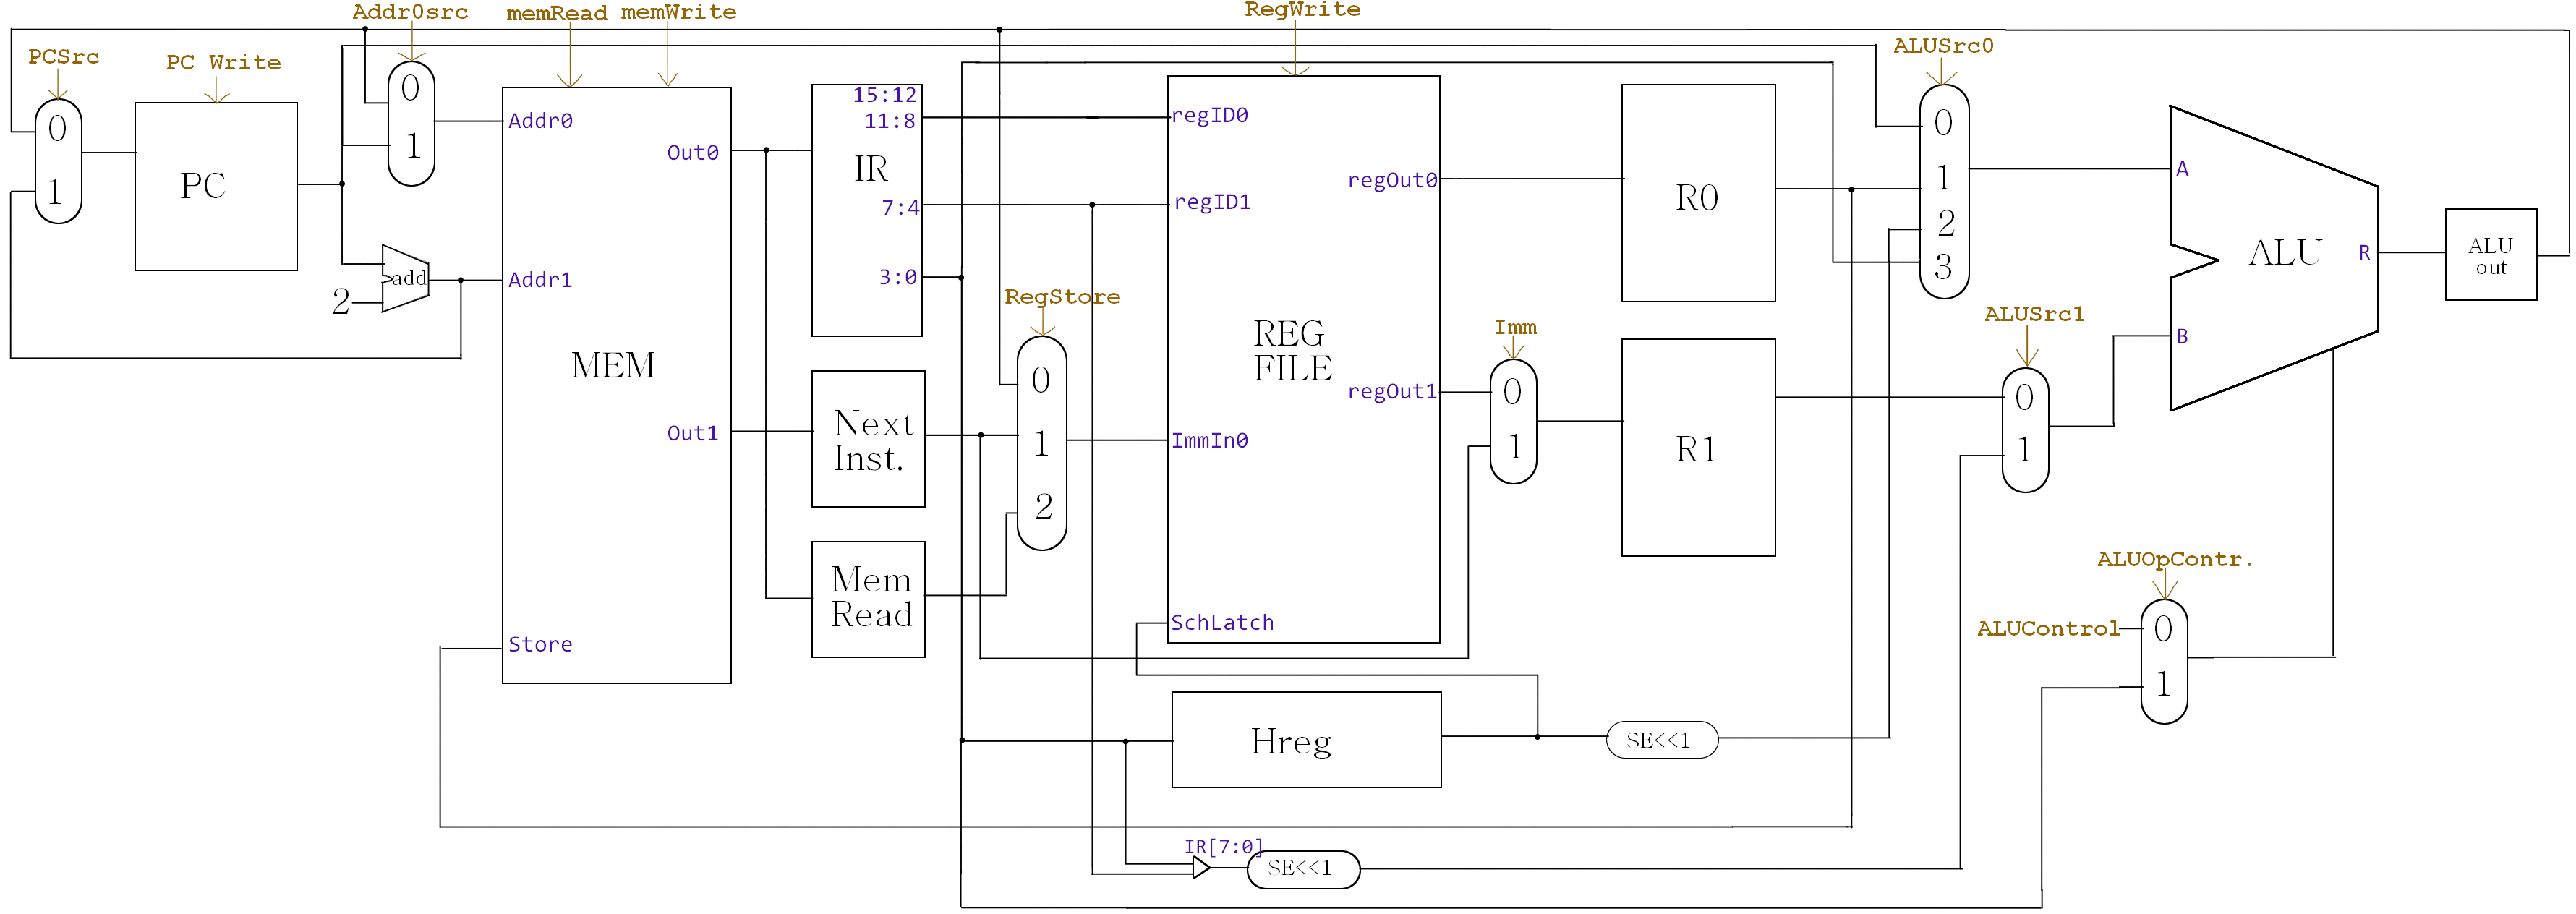
\includegraphics[width=22.5cm]{datapath}
			\end{center}
		\end{landscape}
	\subsection{Unit Tests and Implementation}
		\subsubsection{Single 16-bit Registers}
			\begin{tabular}{ r  r  p{12cm} }
					Implementation: & \multicolumn{2}{l}{Use Micah's 16 bit register}\\
					                &    & \\
					         Tests: & 1. & Pass in a 16-bit value with writing enabled $\Rightarrow$ The whole value should be stored\\
					                & 2. & Pass in a 16-bit value with writing disabled $\Rightarrow$ The none of the value should be stored\\
			\end{tabular}
		\subsubsection{Single 4-bit Registers}
			\begin{tabular}{ r  r  p{12cm} }
					Implementation: & \multicolumn{2}{l}{Use Micah's 16 bit register and change it to only hold 4 bits}\\
					                &    & \\
					         Tests: & 1. & Pass in a 4-bit value with writing enabled $\Rightarrow$ The whole value should be stored\\
					                & 2. & Pass in a 4-bit value with writing disabled $\Rightarrow$ The none of the value should be stored\\
			\end{tabular}
		\subsubsection{SE$<<$1}
		\subsubsection{16-bit Adder}
		\subsubsection{ALU}
		\subsubsection{Register File}
		\subsubsection{Main Memory}
	\subsection{Integration Tests}
	\subsection{Plan Tests}
		\subsubsection{A-Type}
			\begin{tabular}{ r  r  p{12cm} }
					No Immediate:   & 1. & Get this instruction\\
					                & 2. & Increase PC by 2 for the next instruction\\
					                & 3. & R0 and R1 should be loaded with the values from the first and second register in the instruction\\
					                & 4. & The ALUout should have the value of the two values combined using the function code that was passed in\\
					                & 5. & That value should be in the first specified register for the instruction\\ 
					                &    & \\
					With Immediate: & 1. & Get this and the next instruction\\
					                & 2. & Increase PC by 2 for the next instruction\\
					                & 3. & R0 should be loaded with the value from the first register in the instruction and R1 should have the immediate which was in NextInst, PC should have been increased by 2 again\\
					                & 4. & The ALUout should have the value of the two values combined using the function code that was passed in\\
					                & 5. & That value should be in the first specified register for the instruction, the immediate should also have been stored in the second register from the instruction if it was given\\
			\end{tabular}
		\subsubsection{B-Type}
			\begin{tabular}{ r  r  p{13cm} }
					Branches: & 1. & Get this instruction\\
					          & 2. & Increase PC by 2 for the next instruction\\
					          & 3. & R0 and R1 should be loaded with the values from the first and second register in the instruction\\
					          & 4. & The ALUout should have the new PC value for use if the branch is supposed to branch\\
					          & 5. & ALUout should be transferred to PCtemp, the combination of R0 and R1 should be in ALUout\\
					          & 6. & If ALUout is 0 PC should have been changed to what is in PCtemp\\
					          &    & \\
					Read:     & 1. & Get this instruction\\
					          & 2. & Increase PC by 2 for the next instruction\\
					          & 3. & R0 and R1 should be loaded with the values from the first and second register in the instruction, Hreg should have the offset from the instruction\\
					          & 4. & The ALUout should have the value of what's in R1 added to the sign extended, shifted to the left by one value in Hreg\\
					          & 5. & ALUout should be passed into main memory and the value at that address should be in MemRead\\
					          & 6. & The first register specified in the instruction should have the value from memory\\
					          &    & \\
					Write:    & 1. & Get this instruction\\
					          & 2. & Increase PC by 2 for the next instruction\\
					          & 3. & R0 and R1 should be loaded with the values from the first and second register in the instruction, Hreg should have the offset from the instruction\\
					          & 4. & The ALUout should have the value of what's in R1 added to the sign extended, shifted to the left by one value in Hreg\\
					          & 5. & ALUout should be passed into memory as well as the value in R0, the value in R0 should be in memory at that address
			\end{tabular}
		\subsubsection{H-Type}
			\begin{tabular}{ r  r  p{12cm} }
					Schwap: & 1. & Get this instruction\\
					        & 2. & Increase PC by 2 for the next instruction\\
					        & 3. & Hreg should get the schwap group number\\
					        & 4. & SchLatch should now be set to the new schwap group number\\
					        &    & \\
					Sudo:   & 1. & Get this instruction\\
					        & 2. & Increase PC by 2 for the next instruction\\
					        & 3. & Hreg should get the sudo code number\\
					        & 4. & The correct action should now be performed based on the code number\\
			\end{tabular}
		\subsubsection{J-Type}
			\begin{tabular}{ r  r  p{12cm} }
					jr: & 1. & Get this instruction\\
					    & 2. & Increase PC by 2 for the next instruction\\
					    & 3. & PC should be changed to the value in R0 added to the sign extended, shifted to the left by one value in IR[7:0]\\
			\end{tabular}
\section{Assembler and Coding Practices}
	\subsection{Assembler}
		\begin{enumerate}
			\item The order of the parameters for "r" must be flipped.  The hardware expects the memory location in the 2nd register, not the first as in the syntax.
		\end{enumerate}
	\subsection{Code}
		\begin{enumerate}
			\item Avoid branching up and more than 16 instructions down.  The hardware implementation of branching limits branching to only going down a maximum of 16 instructions, but the assembler will convert these to a combination of a branch and jump.
			\item Schwap groups are not preserved across calls.
		\end{enumerate}
\section{Examples}
	\lstset{language=sh}
	\subsection{Basic Use Examples}
		\subsubsection{Loading an immediate into a register}
			\begin{lstlisting}[frame=single]
cpy $t0 32	# Loads 32 into t0
			\end{lstlisting}
		\subsubsection{Making a Procedure Call}
			\begin{lstlisting}[frame=single]
rsh 8		# Switch to arguments schwap
cpy $h0 $t0	# Put argument0 in
cpy $h1 $s1	# Put argument1 in
# Store any wanted temporaries somewhere
jal Call
rsh 9		# Switch to return values schwap
cpy $s0 $h0	# Copy the return values out
			\end{lstlisting}
		\subsubsection{Iteration and Conditionals}
			This is an example of which will iterate over 4 array elements in memory and add 32 to each of them.  It will stop repeating after the 4 elements using beq.
			\begin{lstlisting}[frame=single]
	# There is a base memory address for an array in memory at s0
	cpy $t0 8
	cpy $t1 $z0
loop:
	r   $t2 0($s0)
	add $t2 32
	w   0($s0) $t2
	add $t1 2
	beq $t0 $t1 loop
			\end{lstlisting}
	\subsection{relPrime and gcd Implementation}
		\subsubsection{Assembly}
			\begin{lstlisting}[frame=single]
RelPrime:
	rsh	8		#set schwap
	cpy	$s2 $ra		#save $ra
	cpy	$s0 $h0		#copy n out of schwap
	cpy	$s1 0x2		#load 2 to m
	rsh	8		#set schwap to args
While:
	cpy	$h0 $s0		#set a0 to n
	cpy	$h1 $s1		#set a1 to m
	jal	GCD		#call GCD
	rsh	9		#set schwap
	cpy	$t0 0x1		#load immediate 0x1 to t0
	bne	$h0 $t0 Done	#branch to done if r0 != 1
	add	$s1 0x1		#add 1 to m
	j	While		#jump to the start of the loop
Done:
	rsh	9		#load return registers
	cpy	$h0 $s1		#set r0 to m
	j	$s2 0		#return to the previous function
			\end{lstlisting}
			\begin{lstlisting}[frame=single]
GCD:
	rsh	8		#schwap to argument register
Base:
	bne	$h0 $z0 GMain	#a!=0 go to GMain
	cpy	$t0 $h1		#copy h1 to t0 for RSH
	rsh	9		#schwap to return registers
	cpy	$h0 $t0		#load t0 to r1
	j	$ra 0		#return
GMain:
	beq	$h1 $z0 Exit	#jump to exit if b is zero
	bgt	$h0 $h1 If	#jump to If if a>b
Else:
	sub	$h1 $h0		#else: b=b-a
	j	GMain		#loop
If:
	sub	$h0 $h1		#if: a=a-b
	j	GMain		#loop
Exit:
	cpy	$t0 $h0		#copy h0 to t0 for rsh schwap
	rsh	9		#make sure we're in the right spot
	cpy	$h0 $t0		#copy t0 to h0
	j	$ra		#return
			\end{lstlisting}
	\subsection{Machine Code}
		Machine code for all of the examples will be included once the assembler is complete. 
		\begin{center}
			\begin{tabular}{| c | c || c | c |} \hline
				\multicolumn{2}{| p{1.5cm} ||}{RelPrime} & \multicolumn{2}{ p{1.5cm} |}{GCD} \\ \hline
				PC & Hex  & PC & Hex \\ \hline
				00 & 3009 & 42 & 3009 \\ \hline
				02 & 063F & 44 & 5C05 \\ \hline
				04 & 04CF & 46 & 085F \\ \hline
				06 & 150F & 48 & 300A \\ \hline
				08 & 0002 & 4A & 0A8F \\ \hline
				0A & 3009 & 4C & 2300 \\ \hline
				0C & 0C4F & 4E & 4B05 \\ \hline
				0E & 0D5F & 50 & 1C0F \\ \hline
				10 & 031F & 52 & 0072 \\ \hline
				12 & 300F & 54 & 2C00 \\ \hline
				14 & 1C0F & 56 & 301F \\ \hline
				16 & 0042 & 58 & 6CD7 \\ \hline
				18 & 2C00 & 5A & 0DC2 \\ \hline
				1A & 301F & 5C & 300F \\ \hline
				1C & 300A & 5E & 1C0F \\ \hline
				1E & 180F & 60 & 004E \\ \hline
				20 & 0001 & 62 & 2C00 \\ \hline
				22 & 4C85 & 64 & 301F \\ \hline
				24 & 1C0F & 66 & 0CD2 \\ \hline
				26 & 000A & 68 & 300F \\ \hline
				28 & 2C00 & 6A & 1C0F \\ \hline
				2A & 301F & 6C & 004E \\ \hline
				2C & 1500 & 6E & 2C00 \\ \hline
				2E & 0001 & 70 & 301F \\ \hline
				30 & 300F & 72 & 08CF \\ \hline
				34 & 1C0F & 74 & 300A \\ \hline
				36 & 000C & 76 & 0C8F \\ \hline
				38 & 2C00 & 78 & 2300 \\ \hline
				3A & 301F \\ \cline{1-2}
				3C & 300A \\ \cline{1-2}
				3E & 0C5F \\ \cline{1-2}
				40 & 2600 \\ \cline{1-2}
			\end{tabular}
		\end{center}
\newpage
\section{Notes}
	\subsection{Registers}
		\subsubsection{Non-Schwappable}
			\begin{enumerate}
				\item \$z0 is reset on the rising edge of each CPU cycle, so it can be used for cycle-temporary storage.
				\item The value in \$pc should always be what the current instruction address is +2.
			\end{enumerate}
		\subsubsection{Schwappable}
			\begin{enumerate}
				\item Possible uses for the reserved for future use groups:
					\begin{center} \begin{tabular}{| c | c | c |} \hline
						Group Number & ID    & Use \\ \hline
						\multirow{4}{*}{10}  & 0 & The constant 1 \\
						             & 1     & The constant -1 \\
						             & 2     & User set constant0 \\
						             & 3     & User set constant1 \\ \hline
						11           & 0 - 3 & I/O for devices 0 - 3 \\ \hline
						12           & 0 - 3 & Syscall values 0 - 3 \\ \hline
						13           & 0 - 3 & Kernel \\ \hline
						\multirow{4}{*}{14}  & 0 & Exception Cause \\
						             & 1     & Exception Status \\
						             & 2     & EPC \\
						             & 3     & Exception Temporary \\ \hline
					\end{tabular} \end{center} 
			\end{enumerate}
	\subsection{Instructions}
		\subsubsection{Types and Layouts}
			\begin{enumerate}
				\item More of the types could be combined, but they will run faster if they are not.
			\end{enumerate}
	\subsection{Alias names}
		\subsubsection{Registers}
			\begin{itemize}
				\item[\$z0:] \$0, \$00, \$zz, \$zero
			\end{itemize}
		\subsubsection{Instructions}
			\begin{itemize}
				\item[orr:] or
				\item[bne:] bnq
			\end{itemize}
\end{document}
